\documentclass{docs}

%--- 基本パッケージ ---%
\usepackage{makecell} % 表のセルの配置
\usepackage{pgfgantt} % ガントチャート作成
\usepackage{tabularx} % 表の幅を調整
\usepackage{here} % 図や表の位置を固定 (H)

%--- 文書情報 ---%
\title{システム提案書}
\renewcommand\theadfont\bfseries

\begin{document}

%%%%%%%%%%%%%%%%%%%%%%%%%%%%%%%%%%%%%%%%%%%%%%%%%%%%%%%%%%%%
% 1. 現状の課題
%%%%%%%%%%%%%%%%%%%%%%%%%%%%%%%%%%%%%%%%%%%%%%%%%%%%%%%%%%%%
\section{現状の課題}\label{sec:issues}
%--- システム開発に至った背景や、解決したい社会課題の概要を記述。---%
2024年に高知県を訪れた県外観光客入込数は、対前年比94.3\,\%、約268,000人減の
4,453,000人と推計され、過去最高である前年に比べて減少とはなりましたが、
過去2番目となりました。
また、観光施設の利用状況において、利用者数が最も
多かったのは「高知県立牧野植物園」で314,883人でした\cite{kochi}。
これらのことから、前年に放映された連続テレビ小説「らんまん」が
観光客の動向に大きく影響を与えていると考えられます。

このように、映像作品やコンテンツは観光誘致において、重要な役割を果たしています。
特に、アニメや漫画の舞台となった「聖地巡礼」は、国内外から多くのファンを
惹きつけ、地域経済に大きな影響を与えるポテンシャルを持ちます。しかし、この
一過性のブームをどのようにして持続的な地域振興に繋げるか、という点が課題と
なっています。
本システムは、聖地巡礼という観光体験を最大化し、観光客と地域事業者を繋ぐことで、
この課題の解決を目指すものです。

これらを踏まえた上で、以下に各ステークホルダーの視点での課題を列挙します。
\subsection{行政の視点}
%--- 行政が抱える課題を箇条書きで記述。---%
\begin{itemize}
	\item \emph{観光の一極集中:}特定の有名な観光地(聖地)に
	観光客が集中し、県内他地域への周遊が進まない。結果として、
	地域全体での観光消費額が伸び悩む。
	\item \emph{観光の持続の困難さ:}コンテンツの放送・公開終了後、
	急激に観光客が減少し、ブームが持続しない。一過性のイベントに頼らない、
	継続的な魅力発信が求められる。
	\item \emph{観光動態データの不足:}聖地巡礼に訪れる観光客が「どこから来て」
	「どこを周り」「何に消費しているか」といった詳細な動態データが不足しており、
	効果的な施策立案が困難。
\end{itemize}

\subsection{消費者の視点}
%--- 消費者が抱える課題を箇条書きで記述します。。---%
\begin{itemize}
	\item \emph{情報の散在:} 聖地の場所がWebサイトやSNSに散在しており、
	正確な位置を特定するのが困難。また、古い情報や誤った情報も多い。
	\item \emph{現地での体験価値の低さ:} 現地に到着しても、作中のどのシーンの
	場所なのかが分かりにくい。
	単に風景を見るだけでなく、より没入感のある体験を求めている。
	\item \emph{周辺情報の不足:} 聖地周辺の飲食店や土産物店など、
	ファンならではの視点で楽しめるスポットの情報が不足している。
\end{itemize}


\subsection{事業者の視点}
%--- 事業者が抱える課題を箇条書きで記述.---%
\begin{itemize}
	\item \emph{集客機会の損失:} 聖地巡礼者が店の前を通り過ぎるだけで、
	入店に繋がらない。効果的なアプローチ方法が分からない。
	\item \emph{情報発信の難しさ:} 作品のファンに対して、
	自店の魅力を発信する適切なプラットフォームがない。
	\item \emph{大規模な広告の難しさ:} 大規模な広告は困難であり、
	低コストでターゲット層にリーチできる宣伝手法を求めている。
\end{itemize}

%%%%%%%%%%%%%%%%%%%%%%%%%%%%%%%%%%%%%%%%%%%%%%%%%%%%%%%%%%%%
% 2. 課題解決のための提案
%%%%%%%%%%%%%%%%%%%%%%%%%%%%%%%%%%%%%%%%%%%%%%%%%%%%%%%%%%%%
\section{課題解決のための提案}

%--- 上記の課題をどのように解決するのか、システムのコンセプトを記述
\section{課題解決のための提案}
上記の課題を解決するため、AI(人工知能)とユーザーコミュニティの力を活用した対話型の聖地巡礼サポートシステム「SceneTrip」を提案します。本システムは、特定のIPに依存せず、ファンが主体となって情報を創り上げるプラットフォームとして機能し、持続可能な観光エコシステムの構築を目指します。

\subsection{解決策1: AIによる対話型コンシェルジュ機能}
利用者の「情報の散在」という課題に対し、AIチャットボットが「聖地巡礼に詳しい旅のコンシェルジュ」として対話形式で応えます。
\begin{itemize}
    \item \textbf{パーソナライズされた巡礼プランの提案:} 利用者の興味(作品ジャンル等)、時間、予算に応じて、AIが最適なモデルルートや立ち寄りスポットを提案します。
    \item \textbf{自然言語による情報検索:} 「この近くで、作中に出てきたような雰囲気の喫茶店は?」といった曖昧な質問に対しても、AIが口コミやタグ情報を解析して最適な場所を推薦します。
\end{itemize}

\subsection{解決策2: ゲーミフィケーションとUGCによる周遊促進と体験価値向上}
行政の「周遊促進」と利用者の「体験価値」の課題に対し、ゲーム要素とユーザー生成コンテンツ(UGC)を組み合わせます。
\begin{itemize}
    \item \textbf{実績バッジとランキング機能:} 各聖地や協力店舗へのチェックイン、写真投稿、口コミ投稿といった活動に応じてポイントを付与。特定のクエストをクリアすると「〇〇エリア制覇」などの実績バッジが獲得でき、ランキングで他のユーザーと競うことができます。
    \item \textbf{フォトスポット投稿・共有機能:} ユーザーが「作中のあのシーンのように撮れる」場所や角度を写真付きで投稿・共有。他のユーザーはその情報を元に、より没入感の高い写真撮影体験ができます。
\end{itemize}

\subsection{解決策3: 地域事業者との連携プラットフォームとデータ分析}
事業者および行政の課題に対し、情報発信とデータ活用のプラットフォームを提供します。
\begin{itemize}
    \item \textbf{事業者向け情報発信ツール:} 地域の店舗がアプリ内にクーポンや、ファン向けの特別な商品・サービス情報を簡単に掲載できる機能を提供します。
    \item \textbf{データ駆動型観光の実現:} 利用者の動態データ(個人を特定しない形)を収集・分析し、どのエリアにどのような興味を持つ人が訪れているかを可視化。行政や事業者がデータに基づいた観光施策を立案できるよう支援します。
\end{itemize}

%%%%%%%%%%%%%%%%%%%%%%%%%%%%%%%%%%%%%%%%%%%%%%%%%%%%%%%%%%%%
% 3. 機能概要・前提条件・制約事項
%%%%%%%%%%%%%%%%%%%%%%%%%%%%%%%%%%%%%%%%%%%%%%%%%%%%%%%%%%%%
\section{機能概要・前提条件・制約事項}

\subsection{機能概要}
\subsubsection{利用者向け機能}
\begin{itemize}
	\item AIによる旅行プランサポート(対話型)
\begin{itemize}
	\item 観光地・POI検索
	\item 経路検索
	\item ナビゲーション(ターンバイターン案内)
\end{itemize}
	\item 口コミ・評価
	\item クーポンの受け取り
\end{itemize}

\subsubsection{事業者・行政向け機能}
\begin{itemize}
	\item 広告
	\item 観光動態データ分析
	\item API提供
	\item クーポンの発行
\end{itemize}

\subsection{前提条件}
%--- システムが動作するための前提条件を箇条書きで記述。---%
\begin{itemize}
	\item 利用者がインターネット接続可能なPCまたはスマートフォンを
	所有していること。
	\item 利用者が本システムの利用規約に同意していること。
	\item 一部の機能は会員登録が必須であること。
\end{itemize}

\subsection{制約事項}
%--- システム開発や運用における制約事項を箇条書きで記述。---%
\begin{itemize}
	\item 個人情報保護法を遵守し、情報漏洩を防ぐ仕様であること。
	\item システム管理者による不適切な投稿の監視・削除が可能であること。
\end{itemize}

%%%%%%%%%%%%%%%%%%%%%%%%%%%%%%%%%%%%%%%%%%%%%%%%%%%%%%%%%%%%
% 4. 情報・金銭の流れ
%%%%%%%%%%%%%%%%%%%%%%%%%%%%%%%%%%%%%%%%%%%%%%%%%%%%%%%%%%%%
\section{情報・金銭の流れ}
\subsection{情報の流れ}
%--- システムにおける情報の流れを図で示す。---%
\begin{figure}[H]
	\centering
	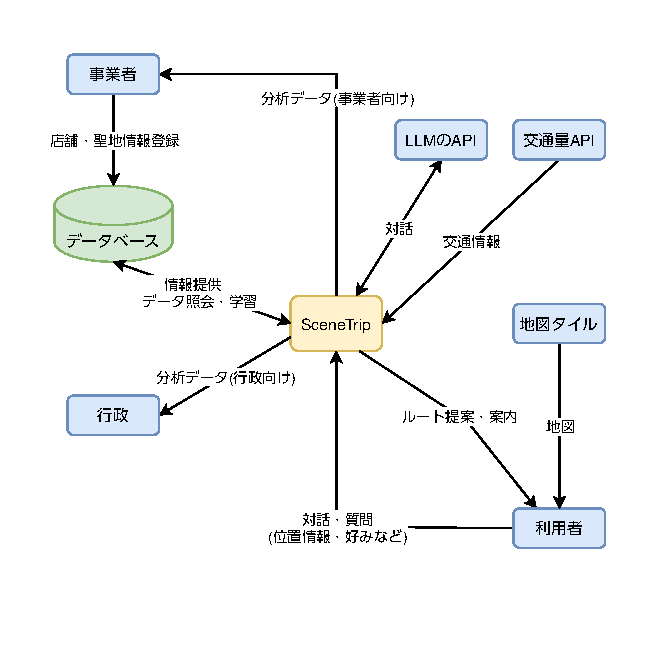
\includegraphics[bb=24.119999 43.253999 266.480711 285.137991,clip]{softinfo.pdf}
	\caption{SceneTripにおける情報の流れ}\label{fig:info}
\end{figure}

\subsection{金銭の流れ}
%--- システムにおける金銭(またはポイント)の流れを図で示す---%
\begin{figure}[H]
	\centering
	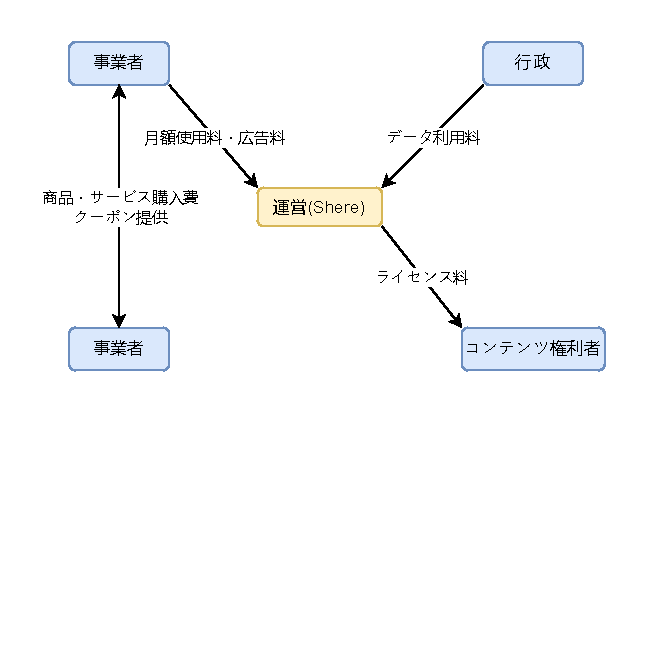
\includegraphics[bb=33.281999 82.403997 272.793718 228.293993,clip]{softmoney.pdf}
	\caption{SceneTripにおける金銭の流れ}\label{fig:money}
\end{figure}


%%%%%%%%%%%%%%%%%%%%%%%%%%%%%%%%%%%%%%%%%%%%%%%%%%%%%%%%%%%%
% 5. 想定する利用者
%%%%%%%%%%%%%%%%%%%%%%%%%%%%%%%%%%%%%%%%%%%%%%%%%%%%%%%%%%%%
\section{想定する利用者}
%--- このシステムの主なターゲットユーザーを箇条書きで記述。---%
\begin{itemize}
	\item 聖地巡礼者
	\item 周遊・体験を重視するアクティブな観光客
	\item デジタルネイティブな情報収集者
\end{itemize}

%%%%%%%%%%%%%%%%%%%%%%%%%%%%%%%%%%%%%%%%%%%%%%%%%%%%%%%%%%%%
% 6. ハードウェア構成・ソフトウェア構成
%%%%%%%%%%%%%%%%%%%%%%%%%%%%%%%%%%%%%%%%%%%%%%%%%%%%%%%%%%%%
\section{ハードウェア構成・ソフトウェア構成}
\subsection{ハードウェア構成}
%--- システムに必要なハードウェア構成を表で示す。---%
\begin{table}[H]
	\centering
	\caption{ハードウェア構成}\label{tab:hardware}
	\begin{tabularx}{0.9\textwidth}{|l|p{9\zw}|X|p{10\zw}|}
		\hline
		\thead{項目} & \thead{種類} & \thead{数量} & \thead{備考} \\ \hline
		メインサーバ & OCI Compute & 1台 & Always Freeサービス(無料枠)\\ \hline
		データベースサーバ & OCI Compute & 1台 & Always Freeサービス(無料枠)\\ \hline
		管理者端末 & PCおよびスマートフォン & 管理者数 & \\ \hline
		利用者端末 & PCおよびスマートフォン & 利用者数 & \\ \hline
	\end{tabularx}
\end{table}

\subsection{ソフトウェア構成}
%--- システムに必要なソフトウェア構成を表で示す。---%
\begin{table}[H]
	\centering
	\caption{ソフトウェア構成}\label{tab:software}
	\begin{tabularx}{0.9\textwidth}{|l|l|X|}
		\hline
		\thead{項目} & \thead{ソフトウェア} & \thead{備考} \\ \hline
		Webサーバ & Nginx & \\ \hline
		データベース & MariaDB & \\ \hline
		バックエンド & PHP(Laravel) & \\ \hline
		フロントエンド & TypeScript & \\ \hline
		端末OS & Android、Linux、Windows、iOS、macOS & \\ \hline
		端末ブラウザ & Firefox、Google Chrome & \\ \hline
		LLM & Google AI Studio & \\ \hline
		地図 & OpenStreetMap & \\ \hline
	\end{tabularx}
\end{table}

%%%%%%%%%%%%%%%%%%%%%%%%%%%%%%%%%%%%%%%%%%%%%%%%%%%%%%%%%%%%
% 7. 運用・保守
%%%%%%%%%%%%%%%%%%%%%%%%%%%%%%%%%%%%%%%%%%%%%%%%%%%%%%%%%%%%
\section{運用・保守}
\subsection{運用}
%--- システムリリース後の日常的な運用業務を箇条書きで記述。---%
\begin{itemize}
	\item システムの稼働監視
	\item 定期的なデータバックアップ
	% \item 口コミ審査
	\item 口コミへの不適切な投稿の監視
	\item セキュリティ監視
	\item 事業者データの登録・管理
	\item 行政への分析データ提供
	\item 問い合わせ対応
\end{itemize}

\subsection{保守}
%--- システムを正常に維持するための保守業務を箇条書きで記述。---%
\begin{itemize}
	\item インフラのメンテナンス
	\item 障害発生時の原因究明と復旧作業
	\item バグや不具合の修正
	\item OSやミドルウェアのアップデート
\end{itemize}

%%%%%%%%%%%%%%%%%%%%%%%%%%%%%%%%%%%%%%%%%%%%%%%%%%%%%%%%%%%%
% 8. 費用対効果
%%%%%%%%%%%%%%%%%%%%%%%%%%%%%%%%%%%%%%%%%%%%%%%%%%%%%%%%%%%%
\section{費用対効果}
\subsection{効果}
%--- システム導入によって得られる定性的な効果を記述。---%
システムの導入により、\cref{sec:issues}に挙げた
各ステークホルダーの視点での課題が解決すると考えられます。

\subsection{収益}
%--- 5年間など、特定の期間における収益モデルと予測金額を記述。---%
収益は、事業者からの月額利用料、広告収入、行政からの手数料を想定します。
\begin{itemize}
	\item \emph{事業者利用料:} $\text{3,000円/月}\times\text{300事業者}
	\times\text{60ヶ月}=\text{54,000,000円}$
	\item \emph{広告収入:} $\text{100,000円/月}\times\text{60ヶ月}
	=\text{6,000,000円}$
	\item \emph{データ利用手数料:} $\text{50,000円/月}\times\text{60ヶ月}
	=\text{3,000,000円}$
\end{itemize}
\emph{5年間の総収益: 63,000,000円}

\subsection{費用}
%--- 開発にかかる初期費用と、運用にかかる費用を表や数式で示します。---%
\begin{itemize}
	\item \emph{初期費用(開発費):}
		\begin{itemize}
			\item 人件費: $\text{10,000,000円/年}\times\text{7名}\times\text{5ヶ月}
			\sim\text{29,166,667円}$
			\item その他(機材費など): 0円\\
			(開発に関わる環境や機材の費用は人件費に含む)
		\end{itemize}
		\emph{初期費用合計: 29,166,667円}
	\item \emph{運用費用(5年間):}
		\begin{itemize}
			\item サーバ費用: $\text{0円/月}\times\text{60ヶ月}
			=\text{0円}$
			\item 維持管理費(人件費など): $\text{2,916,667円/年}\times\text{60ヶ月}
			\sim\text{14,583,333円}$\\
			(年間費用は初期費用の1割として計算)
		\end{itemize}
		\emph{5年間の運用費用合計: 14,583,333円}
\end{itemize}
\emph{5年間の総費用: 43,750,000円}

\subsection{利益}
%--- 5年間など、特定の期間における利益を計算。---%
5年間で得られる利益は以下の通りです。
\begin{gather*}
	\text{総収益} - \text{総費用} = \text{利益}\\
	\text{63,000,000円} - \text{43,750,000円} = \text{19,250,000円}
\end{gather*}

%%%%%%%%%%%%%%%%%%%%%%%%%%%%%%%%%%%%%%%%%%%%%%%%%%%%%%%%%%%%
% 9. 開発体制と工程計画
%%%%%%%%%%%%%%%%%%%%%%%%%%%%%%%%%%%%%%%%%%%%%%%%%%%%%%%%%%%%
\section{開発体制と工程計画}

%--- 開発チームの体制について記述. ---%
本システムの開発は、高知工科大学情報学群の学生7名からなるグループShareが
行います。

%--- 開発スケジュール(ガントチャートなど)を図で示す。---%
また、開発モデルとしてウォーターフォールモデルを採用し、
\cref{fig:gantt}に示す工程で開発します。
\begin{figure}[H]
	\centering
	\begin{ganttchart}[
		canvas/.append style={fill=none,ultra thick},
		title/.append style={fill=none},
		title height=1,
		title label text={\emph{#1}},
		hgrid={draw},
		x unit=16pt,
		y unit chart=34pt,
		bar/.style={},
		bar label node/.append style={align=right},
		left label/.style={
			bar/.style={draw,thick,fill=gray!60},
			bar inline label anchor=west,
			bar inline label node/.style={anchor=east},
			inline,
		},
		right label/.style={
			bar inline label anchor=east,
			bar inline label node/.style={anchor=west},
			inline,
		},
	]{0}{20}
		\gantttitle{2025年}{14}
		\gantttitle{2026年}{7}\\
		\gantttitle{9月}{2}
		\gantttitle{10月}{4}
		\gantttitle{11月}{4}
		\gantttitle{12月}{4}
		\gantttitle{1月}{4}
		\gantttitle{2月}{3}\\
		\ganttbar{要求分析}{0}{0}
		\ganttbar[left label]{10/2}{2}{5}
		\ganttbar[right label]{10/30}{2}{5}\\
		\ganttbar{外部設計}{0}{0}
		\ganttbar[left label]{10/30}{6}{9}
		\ganttbar[right label]{12/1}{6}{9}\\
		\ganttbar{内部設計}{0}{0}
		\ganttbar[left label]{12/1}{10}{12}
		\ganttbar[right label]{12/22}{10}{12}\\
		\ganttbar{コーディング\&\\単体テスト}{0}{0}
		\ganttbar[left label]{12/22}{13}{15}
		\ganttbar[right label]{1/15}{13}{15}\\
		\ganttbar{結合・総合テスト}{0}{0}
		\ganttbar[left label]{1/15}{16}{16}
		\ganttbar[right label]{1/22}{16}{16}\\
		\ganttbar{βテスト}{0}{0}
		\ganttbar[left label]{1/22}{17}{18}
		\ganttbar[right label]{2/5}{17}{18}
	\end{ganttchart}
	\caption{工程計画}\label{fig:gantt}
\end{figure}

%%%%%%%%%%%%%%%%%%%%%%%%%%%%%%%%%%%%%%%%%%%%%%%%%%%%%%%%%%%%
% 参考文献
%%%%%%%%%%%%%%%%%%%%%%%%%%%%%%%%%%%%%%%%%%%%%%%%%%%%%%%%%%%%
\begin{thebibliography}{99}
	%--- 提案書作成にあたり参考にした文献やWebサイトを記述。---%
	\bibitem{kochi}
	高知県,
	“県外観光客入込・動態調査について | 高知県”,
	\url{https://www.pref.kochi.lg.jp/doc/2017090600162/},
	2025年10月20日閲覧.
\end{thebibliography}

\end{document}
